Data mining has contributed numerous techniques for finding patterns in (Boolean) matrices. One fundamental approach is that of \emph{tiling} \parencite{tiling}.  A tile is a rectangular area in a Boolean matrix represented by set of rows and columns such that all values on the corresponding rows and columns in the matrix are equal to 1.  

One is typically not interested in {\em any} tile, but in maximal tiles, i.e., tiles that cannot be extended.  For instance, Figure \ref{tilesExample} shows a binary dataset and two tiles. The first tile consists of the first and second column together with the first and second row. All entries for these rows and columns are 1s. 
Furthermore, it cannot be expanded as adding the third column or row would also include 0 values. The second tile
consists of all three columns and the third row. 
Together these two tiles ``cover'' the whole dataset, that is, all cells with value 1 in the matrix belong to one of the tiles. The area of a set of tiles, denoted as $\textit{area}(\bigT, D)$, is the number of cells (7 in our example) in the (union of the) tiles \bigT occurring in the dataset $D$ 
\begin{figure}[tbh]
  \centering
  \minipage{0.30\textwidth}
  \centering
  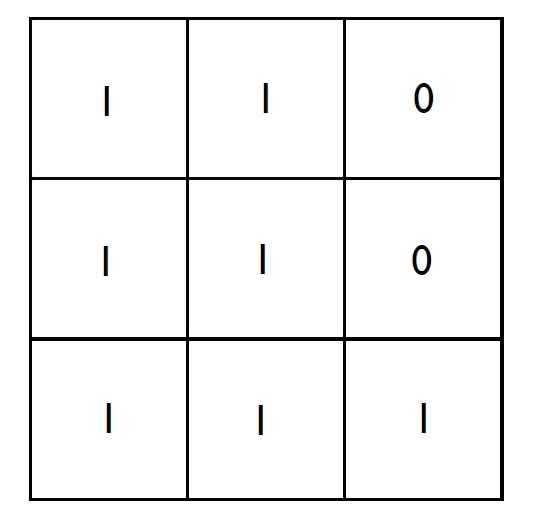
\includegraphics[width=0.5\linewidth]{tile0.jpg}
  \caption*{Initial dataset}
  \endminipage
  \minipage{0.30\textwidth}
  \centering
  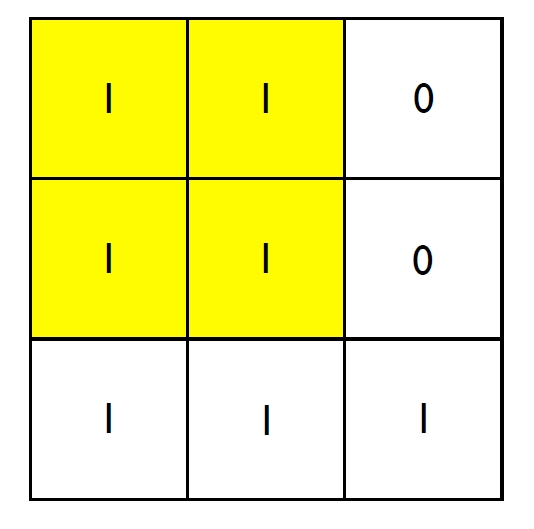
\includegraphics[width=0.5\linewidth]{tile2.jpg}
  \caption*{First tile}
  \endminipage
  \minipage{0.30\textwidth}%
  \centering
  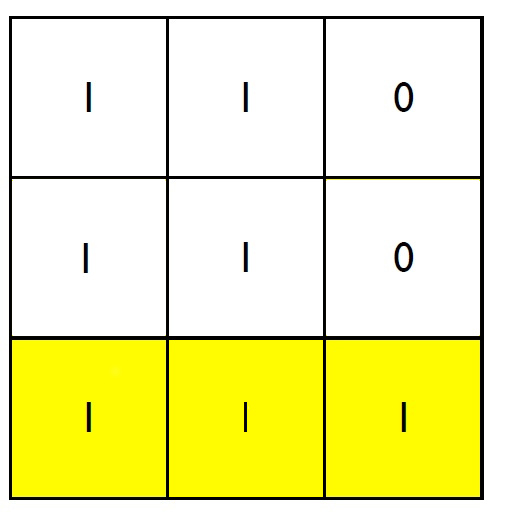
\includegraphics[width=0.5\linewidth]{tile1.jpg}
  \caption*{Second tile}
  \endminipage
  \caption{Example of Boolean tiles and their coverage}
  \label{tilesExample}
\end{figure}



\begin{definition}[Maximum $k$-tiling]
Given a binary dataset $D$ and a positive integer $k$, find a tiling \bigT consisting of at most $k$ tiles and maximizing $\textit{area}(\bigT, D)$.
\end{definition}

We now formalize tiling as a relational data factorization problem and then solve it using ASP. Rather than restricting ourselves to Boolean values as in the traditional formulation, we consider the relational case. The standard way of dealing with tables in attribute-value datasets was to expand them into a sparse Boolean matrix (with one Boolean for every attribute-value). In contrast, our formulation employs the attribute-value format directly. 

%This also allows us to account for the {\tt car} example of Section \ref{decompositionExampleFigure}.

Given a relation \dbvars, denoting that transaction \transaction has \letter for \column, the task is to find a set of tiles that can be applied to the transactions to summarize the dataset \db. Here, a tile is a set of attribute-value pairs.

\begin{figure}[tbh]
	\centering
	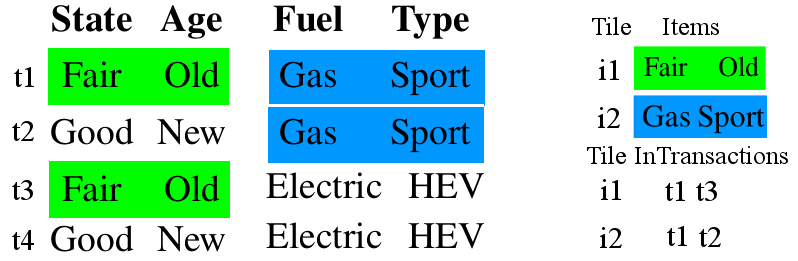
\includegraphics[width=.65\textwidth]{visualTiles.png}
	\caption{Relational tiling: two relational tiles (right) in a toy dataset (left) concerning cars.}
	\label{decompositionExampleFigure}
\end{figure}

In Figure \ref{decompositionExampleFigure}, for example, we can see the initial dataset, in which \textit{State} is an attribute and \textit{Fair} and \textit{Good} are values for this attribute.  Moreover, the blue and green areas indicate two relational tiles occurring in particular sets of transactions.

The two example tiles can be expressed as
\begin{align*}
   &\code(i_1,\textit{fair}, \textit{state}).~\code(i_1,\textit{old}, \textit{age}). ~\inrel(i_1,t_1). ~\inrel(i_1,t_3).\\
   &\code(i_2,\textit{gas}, \textit{fuel}).~\code(i_2,\textit{sport}, \textit{type}). ~\inrel(i_2,t_1). ~\inrel(i_2,t_2).
\end{align*}
where the first argument of each \code is the index of the tile, the second is the value of the attribute, and the third argument is the name of the attribute.
When tile $I$ is applied to a transaction $T$ (i.e., it occurs in the transaction), this is denoted by $\inrel(I,T)$. We call a set of tiles a \textit{tiling}.

We would like to factorize the initial dataset, 
represented as a set of $\db(\textit{fair}$, $\textit{state}, t_1)$, $\db(\textit{old},\textit{age},t_1)$, $\dots$,
using the following \textit{shape} query:
\begin{equation}
  \appr(\column,\letter,\transaction) \leftarrow \code(\indexvar,\letter, \column), \inrel(\indexvar,\transaction). %\text{~\footnotemark}
  \label{tilingshape}
\end{equation}
To reason about the coverage of the shape, i.e., which transactions and attributes are covered in the dataset (indicated by color in Figure \ref{decompositionExampleFigure}), we use the following definition: 
\begin{equation*}
  \covered( \transaction,\column) \leftarrow \appr(\column,\letter,\transaction). %\label{coverapprox}
\end{equation*}
For instance, $\covered(t_1,\textit{age})$ holds because $\code(i_1,\textit{old},\textit{age})$ and $\inrel(i_1,t_1)$ hold. 

To specify the maximum k-tiling problem, we need the following constraints.
\begin{description}
  \item[\onevalueConstraint:] for every attribute of a tile there is at most one value:
\begin{equation}
  \leftarrow \code(\indexvar,\textit{Val}_1, \column),\code(\indexvar,\textit{Val}_2, \column),\textit{Val}_1\neq \textit{Val}_2.  \label{def:tiling_conjunctive} 
\end{equation}
\item[\intersectionConstraint:] tiles do not overlap in the same transaction %(this constraint mimics LCM-$k$ behaviour \cite{tiling}, which only lets new tiles to only work on the uncovered area):
\begin{equation}
\leftarrow \inrel(I_1,T), \inrel(I_2,T), \code(I_1,V,A), \code(I_2,V,A), I_1 \neq I_2. \label{def:non_intersect} 
\end{equation}
  \item[\overcoverageConstraint:] tiles cannot ``overcover'' the transaction, that is, they are only allowed to cover tuples that are in the dataset;   
\begin{equation}
\leftarrow  \code(\indexvar,\letter, \column),\inrel(\indexvar,\transaction), \textit{not } \db(\letter, \column, \transaction). \label{def:pure_tiling}
\end{equation}
\item[\ktiles:] there are at most $k$-tiles (numbered from 1 to $k$): 
\begin{equation*}
   \indexvar = 1 \vee \indexvar = 2 \vee \dots \indexvar = k \leftarrow \code(\indexvar,\letter, \column).%  \label{eq:fixed_tiling}
\end{equation*}
\end{description}
Furthermore, the maximum k-tiling problem searches for the k tiles that maximize the area. This leads to an instance of the $\opti$ score defined by
  \begin{equation}
\maxcover: \quad \#\{ (T,A) : \covered(T,A) \}.  \label{eqn:coverage-opt} 
  \end{equation}
  The statement above correspond to the standard mathematical function optimization notation, that reads as follows: count (\#) the cardinality of the set ($\{ \cdot \}$) of tuples $(T,A)$ such that ($:$) $\covered(T,A)$ holds. When we translate this statements into ASP formulation we have to use special syntax of ASP (\textit{\#maximize}) to capture this mathematical formulation.
 
We specify the high-level model for maximum $k$-tiling in Listing \ref{lst:maxtiling:model}.
\begin{lstlisting}[style=model,label=lst:maxtiling:model,caption=Maximum $k$-Tiling ReDF Model]
 @\textbf{Input:}@ dataset @\db@and constant @$K$@
 @\textbf{Shape:}@ @$\appr(\column,\letter,\transaction) \leftarrow \code(\indexvar,\letter, \column), \inrel(\indexvar,\transaction)$@
 @\textbf{Find:}@  the set of ground facts @$\code(\cdot), \inrel(\cdot)$@
 @\textbf{Satisfying:}@@$\intersectionConstraint  \wedge \overcoverageConstraint$@
         @$\wedge~\ktiles \wedge \onevalueConstraint$@
@\textbf{Maximizing:}@ @\maxcover@ @\vspace{-1pt}
 \end{lstlisting}
To illustrate the advantages of our declarative and modular approach, let us consider a small variation of the tiling task, in which tiles may overlap. 
\paragraph{Overlapping tiling}
\begin{figure}[thb]
  \begin{center}
  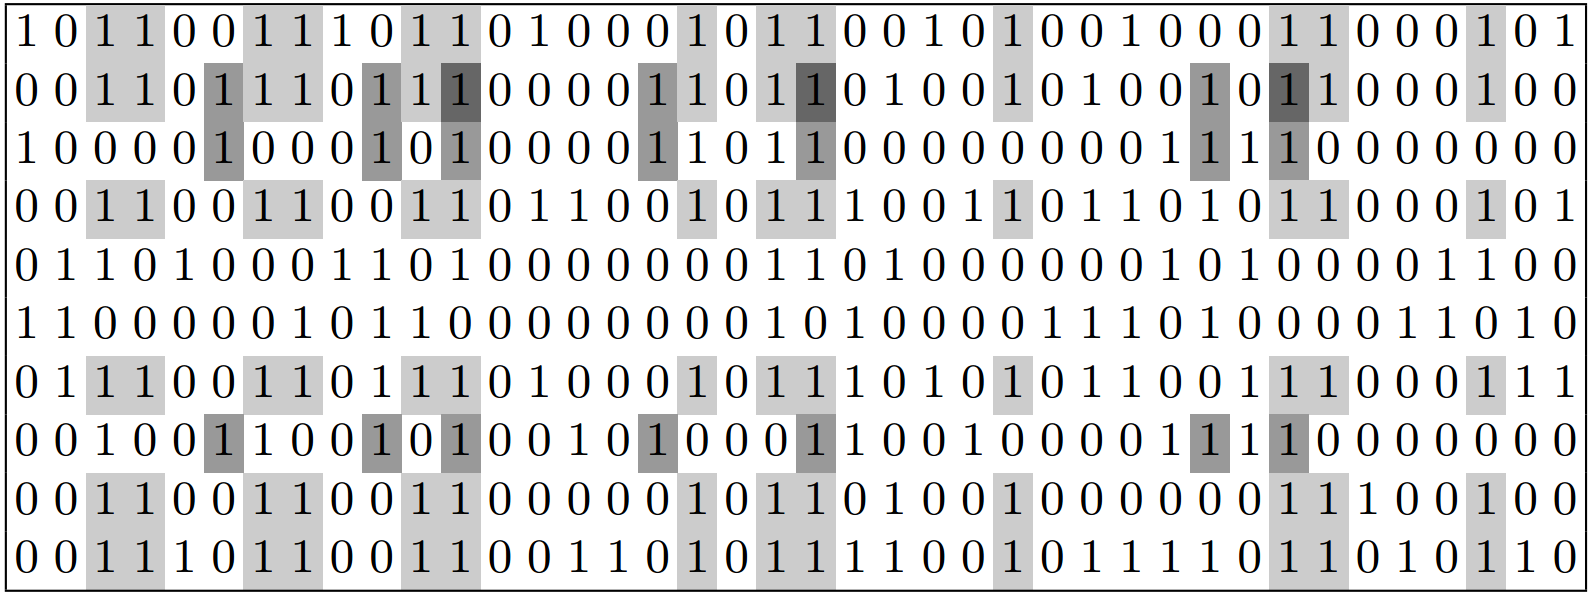
\includegraphics[width=.8\textwidth]{overlapping_geerts.png}
  \caption{Example of a 0/1 database with a tiling consisting of two overlapping tiles\\
  (darkest shaded area corresponds to the intersection of the two tiles), due to \cite{tiling}}
  \label{fig:geerts_overlapping}
\end{center}
\end{figure}
\label{subsubsec:overlapping_tiling}
Figure \ref{fig:geerts_overlapping}, taken from \cite{tiling}, illustrates a Boolean dataset with two overlapping tiles. We investigate and present two new variations of maximum $k$-tiling: overlapping and noisy tiling. The first investigates the global pattern mining task, when the overall coverage is optimized, allowing overlaps between tiles. The second investigates the task when, in $k$-maximum tiling, a tile can have a number of mismatches as covering a transaction. It is straightforward to change the assumption in our ReDF framework (and the corresponding ASP implementation). For the first task, it only involves replacing the constraint \intersectionConstraint by the following constraint.
\begin{description}
\item[\overlappingTilesConstraint:] two tiles in one transaction can intersect only on at most $N$ attributes:
\begin{equation*}
\leftarrow  \inrel(I_1,T), \inrel(I_2,T), \code(I_1,V,A_1), \code(I_2,V,A_2), I_1 \neq I_2, \# \{  A_1 = A_2\} > N.
\end{equation*}
\end{description}
To model the variation that tolerates some noise in the data, we can replace  constraint \overcoverageConstraint by 
\begin{description}
\item[\noiseConstraint:] every tile $I$ can overcover at most \textit{N} attributes in every transaction $T$ where it occurs: %In the algebraic formulation, it would change the \overcoverageConstraint to \noiseConstraint.
\begin{equation*}
\leftarrow  \code(I,V,A),\inrel(I,T), \textit{not}~ \db(V, A, T), \# \{ A \} > \textit{N}.
\end{equation*}
\end{description}
Both variations show that a slight change of the formulation of property of a solution leads to a small change in the modelling and to a small change in the implementation. 

\subsection{The discrete basis problem (DBP) and boolean matrix factorization (BMF)}
\label{subsection:bmf}
BMF has been extensively studied by \cite{conf/icdm/Miettinen12}, resulting in the well-known ASSO algorithm. Let us now show how it can be expressed as ReDF problem. As a starting point we take the same shape (Eq. \ref{tilingshape}) as in the tiling example in Subsection \ref{subsection:tiling}. However, we need to change the constraints to reflect the different properties of the desired solutions: tiles may now overlap, since one is not interested in tiles per se, but in good coverage of the dataset. That is why we remove 
the \intersectionConstraint and \overcoverageConstraint constraints, and introduce a notion of `overcoverage' instead, by means of the following definition:
\begin{equation*}
\overcovered(T,A) \leftarrow  \appr(V,A,T), \textit{not}~ \db(V,A,T). % \rightarrow \textit{overcovered}(T,A). 
\end{equation*}

In the Discrete Basis Problem, the scoring function maximizes the number of covered elements, while minimizing the overcovered ones. The latter term can be simply defined as: 
\begin{description}
\item[\overcoverage:] $\#\{ (T,A) : \overcovered(T,A) \}. $
\end{description}
We specify the high-level DBP model in Listing \ref{dbp:model:full}.
\begin{lstlisting}[style=model, caption=ReDF Model for the Discrete Basis Problem, label=dbp:model:full]
@\textbf{Input:}@ dataset @\db@and constants @$K,\alpha$@
@\textbf{Shape:}@ @$\appr(\column,\transaction) \leftarrow \code(\indexvar,\column), \inrel(\indexvar,\transaction)$@
@\textbf{Find:}@  the set of ground facts @$\code(\cdot), \inrel(\cdot)$@
@\textbf{Satisfying:}@ @$\ktiles$@
@\textbf{Maximizing:}@ @$\maxcover  - \alpha \times \overcover$@
\end{lstlisting}
This formulation mimics \textit{The Discrete Basis Problem} \parencite{dbp}. That is, $K$ plays the role of the basis size and $\alpha$ mimics the bias towards rewarding covering and penalizing overcovering (the flags \texttt{--bonus-covered} and\\\texttt{--penalty-overcovered} in ASSO).
%The correspondence between these two formulations is explained in \ref{subsection:bmf_explanation}.

%Let us reformulate the problem in high algebraic language we used before (assuming the query is the same) \begin{align} & \onevalueConstraint \\ & \ktiles \end{align} Then, the optimization criterion takes into account overcoverage \begin{align} & \opti(M) = \coverage - \overcoverage \end{align}

It is well-known that tiling and {\em Boolean matrix factorization} (BMF) are closely related \parencite{conf/icdm/Miettinen12}. Hence, let us also briefly show how BMF can be realized in our framework.  It corresponds to an instance of DBP where only binary values (true and false) are possible and the \overcoverageConstraint constraint applies. Hence, it is required that the factorization undercovers the initial dataset, i.e., if there is a 0 in a position in the original dataset, then there cannot be a 1 in the approximation.  Therefore, the optimization criterion of DBP is further simplified and we obtain the following BMF model, without overcovering, in Listing \ref{bmf:simplified:model}.
\begin{lstlisting}[style=model, label=bmf:simplified:model, caption=BMF without overcovering]
 @\textbf{Input:}@ dataset @\db@and constant @$K$@
 @\textbf{Shape:}@ @$\appr(\column,\transaction) \leftarrow \code(\indexvar,\column), \inrel(\indexvar,\transaction)$@
 @\textbf{Find:}@  the set of ground facts @$\code(\cdot), \inrel(\cdot)$@
 @\textbf{Satisfying:}@ @$\ktiles \wedge \overcoverageConstraint$@
 @\textbf{Maximizing:}@ @$\maxcover$@ @\vspace{-9pt}@
 \end{lstlisting}


\subsection{Discriminative k-pattern set mining}
\label{subsec:discriminative}
A common supervised data mining task is that of discriminative pattern set mining \parencite{DBLP:conf/pkdd/KnobbeH06}.  Let \dbvars be a categorical dataset, \positiveT (\negativeT) be the set of positive (negative) transactions, and $ k$ the number of tiles. Then, the task is to find extensions of the relations \codevars and \invars such that positive and negative transactions are discriminated. A standard interpretation is to find tiles that cover as many positive and as few negative ones as possible \parencite{Liu98integratingclassification}. The only required change in the model concerns the scoring function (and assigning some weight to the errors):
\begin{equation}
  \#\{T: \covered(T),\positiveT \} - \alpha \#\{ T: \covered(T),\negativeT \}, \label{eq:discriminate_optimization}
\end{equation}
where $\alpha$ is a constant that represents the weights for the errors made. It is typically a domain specific parameter (the cost of covering a negative example by a rule, i.e., the false
positive cost or a weight of a negative example).
Let us denote the coverage of the positive transactions as \coverageplus (left set term in Eq. \ref{eq:discriminate_optimization}) and the coverage of negative as \coverageminus (right set term in Eq. \ref{eq:discriminate_optimization}).  

Given that we have no \overcoverageConstraint constraint and negative transactions can be covered, the optimization criterion is given by
\begin{align*}
  & \opti(T) = \coverage^+ - \alpha \times \coverage^- .
\end{align*}

This corresponds to the high-level model in Listing \ref{lst:discriminative:model}.
\begin{lstlisting}[style=model,label=lst:discriminative:model,caption=ReDF Discriminative Patter Set Mining Model]
 @\textbf{Input:}@ dataset @\db@and constants @$K, \alpha$@
 @\textbf{Shape:}@ @$\appr(\column,\letter,\transaction) \leftarrow \code(\indexvar,\letter, \column), \inrel(\indexvar,\transaction)$@
 @\textbf{Find:}@  the set of ground facts @$\code(\cdot), \inrel(\cdot)$@
 @\textbf{Satisfying:}@ @$\ktiles \wedge \overcoverageConstraint \wedge \onevalueConstraint$@
 @\textbf{Maximizing:}@ @$\coverageplus - \alpha \times\coverageminus$@
\end{lstlisting}
\subsection{Block-diagonal matrix form}\label{subsec:blockdiagonal}
\begin{figure}[t]
\begin{center}
\begin{subfigure}{.32\textwidth}
  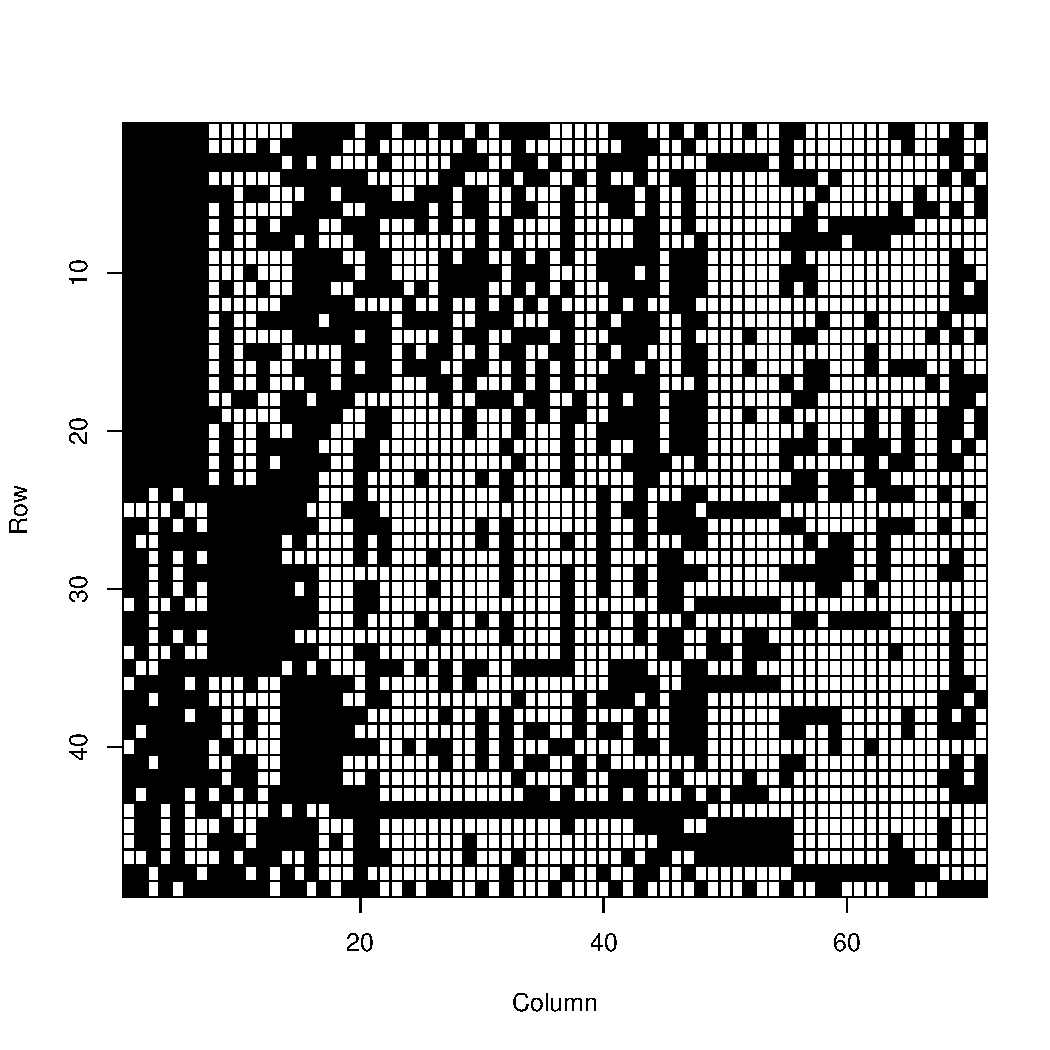
\includegraphics[width=\textwidth]{diagPure.pdf}
  \captionsetup{skip=-5pt}
  \caption{Regular}
  \label{fig:regular_block_diagonal}
\end{subfigure}
   \hfill 
\begin{subfigure}{.32\textwidth}
  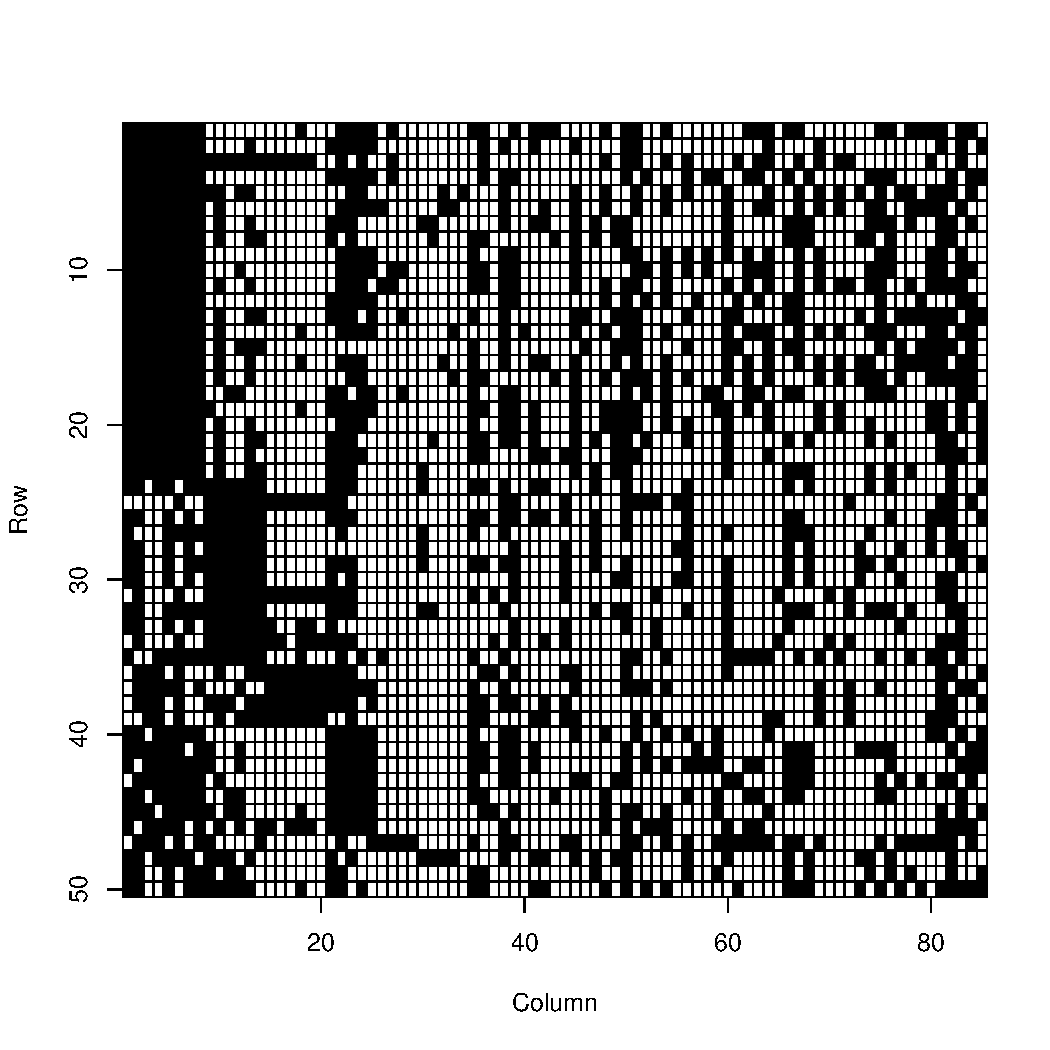
\includegraphics[width=\textwidth]{diagPenalty.pdf}
  \captionsetup{skip=-5pt}
  \caption{With penalties}
  \label{fig:penalty_block_diagonal}
\end{subfigure}
\begin{subfigure}{.32\textwidth}
  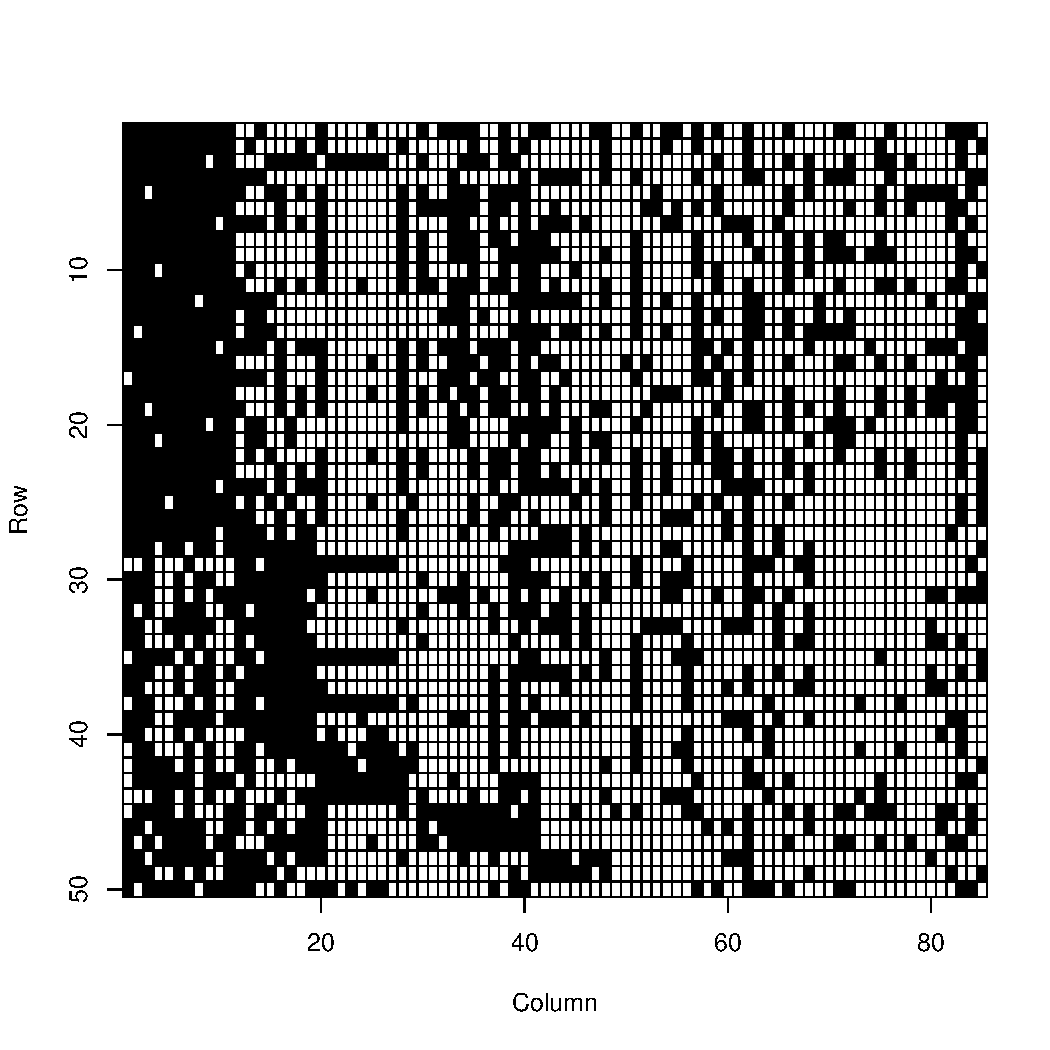
\includegraphics[width=\textwidth]{diagNoisy.pdf}
  \captionsetup{skip=-5pt}
  \caption{With penalties and noise}
  \label{fig:noisy_block_diagonal}
\end{subfigure}
\end{center}
\captionsetup{skip=-8pt}
\caption{Re-arranging a matrix in block-diagonal form (Animals dataset): (a) regular, (b) with penalties, (c) with noisy blocks and penalties}
\label{fig:diag_examples}
\end{figure}

\cite{blockdiagonal} introduced the problem of and an algorithm for permuting the rows and columns of a sparse matrix into block diagonal form. 
They relate this problem to other combinatorial and classical linear algebra problems. The underlying block-diagonal structure of a matrix can be used to parallelize certain matrix computations. An illustration of block-diagonalization (several variants) of the Animals dataset is depicted in Figure \ref{fig:diag_examples}.

We reduce it to a form of tiling. The shape query is the same as in tiling but the constraints are different: if a tile $I_1$ has an attribute $A$, then a tile $I_2$ cannot use the same attribute. A similar constraint is imposed on the $\inrel$ predicate and transactions stating that each item $A$ can belong to only one tile
\begin{description}
\item[\blockedItems:] $\leftarrow \code(I_1,A), \code(I_2,A), I_1 \neq I_2. $
\end{description}
Only one tile can occur in a transaction $T$.
\begin{description}
\item[\blockedTranst:] $\leftarrow  \inrel(I_1,T), \inrel(I_2,T), I_1 \neq I_2. $
\end{description}

We also modify the optimization criterion to take into account elements not covered by a tile but blocked by this tile. Every tile that selects attributes and transactions prohibits other tiles to use these attributes and transactions by means of the \blockedItems and \blockedTranst constraints. We penalize excessive usage of attributes and transactions by a single tile. We do this to improve the block form of the matrix, since in this task we are not just interested in a tiling with maximal coverage, but in a tiling that maximizes the number of elements on the diagonal and minimizes the number of elements everywhere else. To enforce this we introduce two functions:

\begin{description}
\item[\itemPenalty:] $\#\{ (T,A) : \appr(T,A'), ~\textit{not } \covered(T,A) \}$
\end{description}

\begin{description}
\item[\transactionPenalty:] $\#\{ (T,A) : \appr(T',A), ~\textit{not } \covered(T,A) \}$
\end{description}

Then, the whole problem is formulated in Listing \ref{lst:blockdiagonal:model}.
\begin{lstlisting}[style=model, label=lst:blockdiagonal:model, caption=ReDF Block-Diagonal Model]
@\textbf{Input:}@ dataset @\db@and constants @$N,\alpha,\beta$@
@\textbf{Shape:}@ @$\appr(\column,\letter,\transaction) \leftarrow \code(\indexvar,\letter, \column), \inrel(\indexvar,\transaction)$@
@\textbf{Find:}@  the set of ground facts @$\code(\cdot), \inrel(\cdot)$@
@\textbf{Satisfying:}@ @$\blockedTranst \wedge \blockedItems $@
              @$\onevalueConstraint \wedge \noiseConstraint \wedge \intersectionConstraint$@
@\textbf{Maximizing:}@ @$\coverage -\alpha \times \transactionPenalty - \beta \times \itemPenalty$@
\end{lstlisting}


If we omit \itemPenalty and \transactionPenalty, we obtain the standard optimization function for tiling. In the experimental section we evaluate the effect of the presence of this penalty. 



